\documentclass[a4paper,10pt]{article}
\usepackage[utf8]{inputenc}
\usepackage{amsmath}
\usepackage{graphicx}
\usepackage{epsfig}
\usepackage[english]{babel}
\usepackage{url}
\usepackage{epstopdf}
\usepackage{subfig}
\usepackage{graphicx}
\usepackage{enumerate}
\usepackage{appendix}
%\usepackage{anysize}
%\marginsize{1cm}{1cm}{1cm}{1cm}
\title{\textit{IEE3853} Detectores para Astronomía (I-2012)}
\author{\textbf{Tarea 04 – Diseño del sistema de detección para un Imager} \\Norman F. Sáez\\nfsaez@uc.cl}

\date{2012/07/07}

\begin{document}
%\input{portada}
\maketitle
\section*{Introducción}

El presente documento especifica sistema de detección para el telescopio ESO 1
metro, en donde el instrumento a utilizar es Imager.  Los requerimientos
especificados fueron los siguientes:

\begin{itemize}
\item Especificar el CCD científico a utilizar.

\item Predecir readout noise, dark current y readout time.

\item Estimar si el diseño óptico es adecuado o es preferible modificarlo, para
el detector seleccionado. En caso de modificación, especifique los
requerimientos para el nuevo diseño óptico.

\item Estimar los tiempos de exposición para diversos filtros considerando la
eficiencia cuántica del CCD seleccionado y la obtención de una SNR de al menos
10. Analice filtros del tipo SDSS4 (Sloan Digital Sky Survey) para su análisis.

\item Especificar los requerimientos de enfriamiento criogénico, en particular
temperatura de operación. Sugerir posibilidades de criogenia.
\end{itemize}

Las siguientes secciones muestran como se intenta satisfacer las necesidades que se especificaban en la tarea.


\section{Especificar el CCD científico a utilizar}
Parámetros del sistema:
\begin{itemize}
\item Field of View del instrumento = $14 '$
\item Diámetro Plano Focal = $30.8 [mm]$
\item Escala en el plano focal = $\frac{FoV}{Diametro\ Plano\ Focal} = 0.4545 ['/mm]$
\item Field of View requerido: $5'$ en x
\item Field of View requerido: $5'$ en y
\item Dimensiones del detector: $\frac{5'}{0.4545['/mm]} = 11 [mm]$ en x
\item Dimensiones del detector: $\frac{5'}{0.4545['/mm]} = 11 [mm]$ en y
\end{itemize}
Entonces el detector debe tener un tamaño de $11x11[mm]$.  Tamaño imagen de la
PSF en el plano focal: $\frac{0.00833'}{0.4545 ['/mm]} = 0.01833[mm] = 18.33516
[\mu m]$, utilizando el dato de Optimal Sampling, podemos obtener cuanto tiene
que ser el tamaño del píxel: $\frac{18.33516}{3} = 6.111 [\mu m]$.

Con los datos obtenidos, se necesita como mínimo:
\begin{itemize}
\item CCD $11x11[mm]$.
\item Tamaño de píxel $6.11 [\mu m]$.
\end{itemize}

Con estos datos no es posible tener un CCD desde la pagina del proveedor. Por
lo que se intentara buscar uno similar y ajustar algunos parámetros del
instrumento.

La primera es ser mayor al tamaño mínimo de CCD necesario

La segunda es tener pixeles que sean menores al tamaño máximo

Es que el CCD sea menor al diámetro del plano focal. Los datos son reflejados
en figura \ref{fig:p1} 
\begin{figure}[ht!]
  \centering
  \subfloat[Tabla de datos siguiendo especificaciones]{\label{fig:p1_a}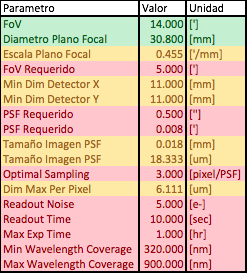
\includegraphics[width=0.5\textwidth]{img/img1}}
  ~ 
  \subfloat[Simbologia]{\label{fig:p1_b}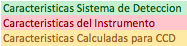
\includegraphics[width=0.3\textwidth]{img/img3}}
  ~ 
  \caption{Tabla de datos y simbologia de acuerdo a las especificaciones}
  \label{fig:p1}
\end{figure}



\section{Estimar si el diseño óptico es adecuado o es preferible
modificarlo,para el detector seleccionado. En caso de modificación, especifique
los requerimientos para el nuevo diseño óptico.} Dado que no existian CCD que
calzaran con las especificaciones, se plantea la siguiente solucion:
\begin{itemize}
\item Disminuir escala en el plano focal del instrumento
\end{itemize}

Para ello, se necesita:
\begin{itemize}
\item Disminuir el Field of View
\end{itemize}

Otra opcion es aumentar el diametro, pero como se tiene muchisimo field of
view, se descarta esta solucion. Luego, se ajusta se seleccionaron camaras que
tuvieran el diametro focal cercano a 30.8. Las mejores camaras escogidas
fueron:
\begin{itemize}
\item CCD40-42
\item CCD50-30
\end{itemize}

Se escoje CCD50-30 debido a su mayor \textit{Image area}  ($28.17 x 25.92 mm$)
. Field of View fue ajustado para y se verifica las nuevas especificaciones del
detector, como se puede apreciar en la figura \ref{fig:p2}
\begin{figure}[ht!]
  \centering
  \subfloat[Tabla de datos ajustando especificaciones]{\label{fig:p2_a}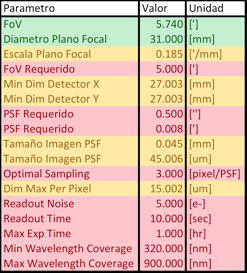
\includegraphics[width=0.5\textwidth]{img/img2}}
  ~ 
  \subfloat[Simbologia]{\label{fig:p2_b}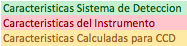
\includegraphics[width=0.3\textwidth]{img/img3}}
  ~ 
  \caption{Tabla de datos ajustada y simbologia}
  \label{fig:p2}
\end{figure}

\section{Predecir readout noise, dark current y readout time}
Dada las caracteristicas que se ocuparon en la pregunta 2, y de acuerdo a la tabla presentada en figura \ref{fig:p2}
\section{Estimar los tiempos de exposición para diversos filtros considerando la
eficiencia cuántica del CCD seleccionado y la obtención de una SNR de al menos
10. Analice filtros del tipo SDSS4 (Sloan Digital Sky Survey) para su análisis.}

\section{Especificar los requerimientos de enfriamiento criogénico, en particular
temperatura de operación. Sugerir posibilidades de criogenia.}


\end{document}

